\documentclass[conference]{IEEEtran}
\IEEEoverridecommandlockouts
% The preceding line is only needed to identify funding in the first footnote. If that is unneeded, please comment it out.
\usepackage{cite}
\usepackage{amsmath,amssymb,amsfonts}
\usepackage{algorithmic}
\usepackage{graphicx}
\usepackage{textcomp}
\usepackage[brazilian]{babel}
\usepackage[utf8]{inputenc}
\usepackage[T1]{fontenc}
\usepackage{program}


\def\BibTeX{{\rm B\kern-.05em{\sc i\kern-.025em b}\kern-.08em
    T\kern-.1667em\lower.7ex\hbox{E}\kern-.125emX}}
\begin{document}

\title{REDE NEURAL ARTIFICIAL EM SIMULAÇÃO DA OCORRÊNCIA DE FOGO NO CERRADO }
\author{
\IEEEauthorblockN{Letícia Meirelles; Manoel Cardoso}
\IEEEauthorblockA{Instituto Nacional de Pesquisas Espaciais / Centro de Ciência do Sistema Terrestre – INPE/CCST\\
leticia.meirelles@inpe.br; manoel.cardoso@inpe.br}}


\maketitle


 Trabalho apresentado à disciplina Análise de Algoritmo e Estrutura de Dados da UNIFESP, como requisito parcial de avaliação. \\Prof Lilian Berton.\\ Orientador: Manoel Cardoso


%\begin{IEEEkeywords}
 %Cerrado, vegetação, fogo, redes neurais.
%\end{IEEEkeywords}



\section{Introdução}

Existe grande interesse na preservação do Cerrado devido principalmente à sua alta biodiversidade (Myers et al 2000) e potencial de recursos naturais (Nóbrega et al. 2017). Apesar disso, o bioma deverá sofrer com pressões devido à mudanças no clima e em seu uso e cobertura, como a produção de soja e milho, e pastagens (Miranda et al. 2014). Assim, a capacidade de simular a dinâmica do Cerrado pode contribuir em tomadas de decisões sobre sua preservação. Isto inclui o desenvolvimento de métodos para simular a ocorrência do fogo, o que têm uma forte influência na dinâmica da vegetação desta região (Arruda et al. 2018).\\
Neste contexto, esse estudo desenvolve uma aplicação de redes neurais artificiais (Werbos 1975) para simular a ocorrência do fogo a partir de variáveis ambientais calculadas pelo Integrated Land Surface Model (INLAND, baseado em Foley et al. 1998). O INLAND oferece a capacidade de simular a dinâmica do Cerrado sob diferentes condições climáticas e de uso na terra, e explorar mecanismos de interação entre a atmosfera e a superfície da região.\\
A presente metodologia e objetivos se concentram em validar a possibilidade de uso de redes neurais artificiais como suporte de cálculo da ocorrência natural de fogo a partir de saídas do INLAND em simulações da dinâmica de vegetação, pelas informações que o modelo provém sobre biomassa vegetal e umidade do solo. Além destas informações, são também utilizados dados meteorológicos de precipitação e velocidade do vento, e detecções de fogo pelo sensoriamento remoto com o Moderate Resolution Imaging Spectroradiometer (MODIS).

\section{Metodologia}
Como ferramentas principais para implementação da rede neural foram utilizados resultados do modelo INLAND e dados de focos de queimadas do produto MODIS MCD14ML (University of Maryland, EUA, http://modis-fire.umd.edu). O INLAND é desenvolvido no CCST/INPE com base em Foley et al. (1996), e simula as características dominantes da superfície vegetada continental, com resolução espacial de 50km, e em escala temporal de dias-anos. O modelo integra processos superficiais que representam os efeitos do clima na superfície (como crescimento ou mortalidade da vegetação), e da superfície no clima (como evapotranspiração e reflexão da energia solar), e permite considerar cenários de desmatamento e agricultura.\\ 
Para obtenção dos resultados com o INLAND, realizou-se uma simulação no domínio de território do Brasil para um período total de 110 anos. A fim de se evitar efeitos de condições iniciais, a extração de valores simulados se concentrou nos últimos 10 anos apenas. A configuração desta simulação contempla a dinâmica de vegetação, concentração de CO2 estática, e dinâmica de uso da terra desativada. Os dados de entrada sobre condições atmosféricas correspondem a uma climatologia de trinta anos (1961 a 1990) gerada a partir de dados do CRU (Climate Research Unit, Global Climate Dataset).\\  


\subsection{Algoritmo Implementado}

Para o desenvolvimento da Rede Neural Artificial (RNA) multicamadas no cálculo de ocorrência de fogo foi utilizado a linguagem de programação Python, treinadas com o algoritmo backpropagation (Werbos, 1975). A topologia da rede a ser utilizada consistem em 3 camadas (camada de entrada, camada oculta e camada de saída). Foram considerados  11 neurônios para as camadas de entrada; 2,3,5,10 e 100 neurônios na camada oculta; e 1 neurônio para a camada de saída.\\
O algoritmo de rede neural artificial multiplas camadas com retroalimentação consiste na inicialização dos pesos de cada neurônio com valores aleatórios, repete o treinamento da série de amostras até que as saídas satisfaçam o critério de parada, a partir do erro quadráticos médio ou atinja o número limite de interações. Para cada elemento da amostra é calculada a saída, e comparada com a esperada, a diferença entre o erro e o valor simulado é utilizado para ajuste dos pesos.\\
%Algoritmo BackPropagation\\
%Inicia todas conexões com valores de pesos aleatórios\\
%Repete\\
   %Para cada amostra na série de treinamento (x,y)\\
    %  Para cada camada i de 1 até N\\
     %    Para cada neurônio j de 1 até Mi\\
    %        Calcular saída fij(x)\\
   %      erro =  y- fij(x)\\
  %    Para cada camada i de N até 1\\
 %        Para cada neurônio j de 1 até Mi\\
  %               Atualizar pesos\\
%Até que (erro < e) ou (número máximo de ciclos)\\

\begin{program}
\mbox{Algoritmo BackPropagation:}
\BEGIN \\ %
\rcomment{Inicia todas conexões com valores de pesos aleatórios}

\DO \IF erro < \varepsilon \OR nEpoca > maxEpoca \THEN \EXIT \FI;
\rcomment{ $\varepsilon$  é média do erro quadrático }

  	\FOR a:k \TO nAmostras step 1 do
		x:= amostra[0:k]
		y:= amostra[1:k]
		\FOR i:1 \TO nCamada \STEP 1 \DO
			\FOR j:1 \TO nNeuronio \STEP 1 \DO
				|fij|(x)\rcomment{calcula saída}
         			erro:=  y- |fij(x)|
			\END
		\END
		\FOR i:nCamada \TO 1  \STEP 1 \DO
			\FOR j:1 \TO nNeuronio \STEP 1 \DO
				|atualizaPesos|(erro)

\end{program}

A Figura~\ref{modelo} apresenta o modelo geral de um neurônio artificial.

\begin{figure}[htbp]
\centerline{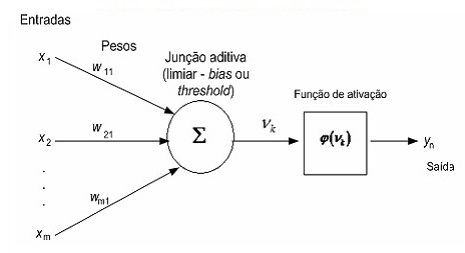
\includegraphics[width=0.4\paperwidth]{figuras/modelo.jpg}}
\caption{Modelo geral de um Neurônio Artificial (HAYKIN, 2001)}
\label{modelo}
\end{figure}

O primeiro da Figura~\ref{modelo} elemento é um conjunto de sinapses ou linha de conexão, cada qual caracterizada por um peso$^{w_{kj}}$, com k = 1 e j = 1,2,..., m.\\
O segundo item da Figura~\ref{modelo} trata da soma dos sinais de entrada, ponderada pelas sinapses do neurônio (combinação linear), onde:\\
\[V _{k}=\sum_{j=0}^{m}W_{kj}X_{j}\]
A função de ativação, Figura~\ref{modelo}, restringe a amplitude de saída de um neurônio, limitando o intervalo de saída para um valor finito.
\[Y _{k}=\varphi (\nu _{k})\]
A equação da função de ativação, para este trabalho usada, tangente hiperbólica assumindo valores entre 1 e -1, onde $\alpha$ é o parâmetro de inclinação da curva, $\beta$ são os limites inferiores e superiores e $\nu$   é o valor de ativação, deste modo:
\[f(v)=a \frac{e^{(bv)}-e^{(-bv)}}{e^{(bv)}+e^{(-bv)}}\]





Para a treinamento da RNA, o total dos dados de amostras foi dividido aleatoriamente em 70\% para o treinamento, 15\% para testes e 15\% para validação. Em cada treinamento foram realizadas até 1440 interações da série de amostras de dados, até que o erro médio quadrático entre a saída desejada e a saída calculada fosse menor que 0.01 e tenha atingido o limite de 1000 treinamentos da série de dados.\\




\subsection{Análise de Complexidade do Algoritmo}
Esta seção apresenta uma análise computacional e de complexidade de mensagens para do algoritmo de rede neural perceptron multiplas camadas (MPL).
 \subsubsection{Complexidade de Espaço}
 A complexidade de espaço em memória de uma rede neural do tipo multiplas camadas é insignificante na maioria das vezes. Em um extremo, uma única interação pode abrigar um neurônio e, portanto, precisa armazenar as estruturas de dados, incluindo entradas, que são saídas de todos os outros neurônios, parâmetros e modelo computacional do neurônio, que coletivamente exigem alocação de espaço de memória.\\
  A estrutura de dados mais dispendiosa é a matriz de entrada de neurônios unidimensional, que crescerá linearmente no número de neurônios, que enviam suas saídas como entradas para um determinado neurônio. Portanto, a complexidade espacial do caso de um neurônio por interação é linear no número de neurônios conectados ao único neurônio em consideração. Se houver múltiplos neurônios alojados por uma única entrada, a complexidade do espaço ainda é linear, pois a complexidade do espaço resquisitado a um único neurônio é multiplicada pelo número de neurônios alojados naquela único interação para determinar a complexidade do espaço resultante.

 \subsubsection{Complexidade de Tempo}
A complexidade de tempo de uma única iteração depende da estrutura da rede reural. Para o algoritmo MLP, o tempo é dado pelas multiplicações de matrizes de entradas das amostras da série e neurônios de cada camada. Considerando a complexidade de um algoritmo para a multiplicação de matrizes, e D e seja o tamanho da lista de entradas. Em uma única camada com dimensão de entrada N dimensão de saída M, as propagações diretas e reversa serão sempre O (N*M*D) assumindo um algoritmo de produto de matriz. Soma-se isto para casa camadas, então pode-se obter o tempo para o calculo de uma interação de um algoritmo de backprotagation. Como a diferenciação em modo reverso é, no máximo, um fator constante mais lento do que o cálculo direto da função de saída da rede neural, todas as outras operações necessárias podem ser calculadas em tempo linear para a série de interações.

\subsection{Dados de Input}
Depois da execução da simulação do INLAND, foi realizado o recorte para a região da Serra do Espinhaço-MG, para longitude -44.75 até -43.25(3 pontos de grade) e latitude -18.25 até -17.25 (4 pontos de grade), escolhido como uma região representativa das condições do Cerrado. A sub-região de estudo totaliza uma área de 12 pontos de grade, onde foram extraídas saídas com frequência mensal. O número total de amostras é equivalente à 10*12*12=1440. Como entradas para a rede neural, foram consideradas para cada amostra as seguintes variáveis: umidade do solo, biomassa total acima do solo, velocidade do vento na superfície, temperatura próxima à superfície, e precipitação média.\\ 
Após o recorte da região, e do período e variáveis das saídas do INLAND foi necessário gerar a matriz de entradas da rede e saídas esperadas. Para cada amostra foi verificado a saída desejada considerando os dados do MODIS para o mês equivalente, colocados em ordem aleatória para prevenção de tendências associadas à ordem de apresentação dos dados. Os dados foram ainda pré-processados através de normatizações e conversões de formato para torná-los mais apropriados à sua utilização na construção da rede.\\ 
As Figuras~\ref{inputFogo},\ref{inputPrec},\ref{inputWsoi},\ref{inputTemp},\ref{inputVento},\ref{inputBioLit} e \ref{inputFrac} apresentam as medias dos valores de dados de saídas do INLAND que foram utilizados como entrada para o treinamento da RNA.\\


\begin{figure}[htbp]
\centerline{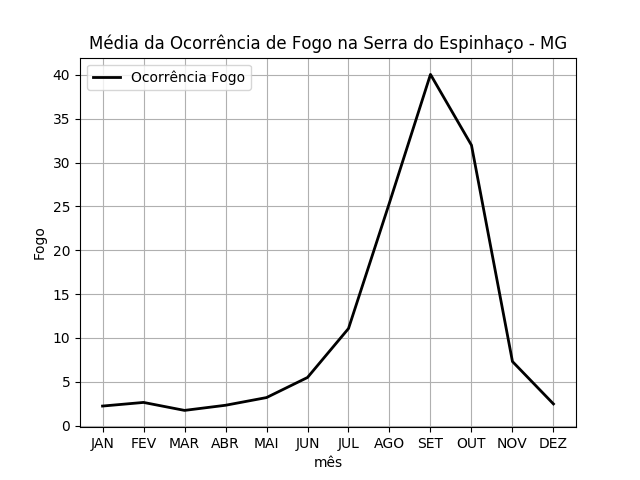
\includegraphics[width=0.4\paperwidth]{figuras/fogo.png}}
\caption{Climatologia da ocorrência de fogo entre 2002 a 2017 na região da Serra do Espinhaço - MG}
\label{inputFogo}
\end{figure}


\begin{figure}[htbp]
\centerline{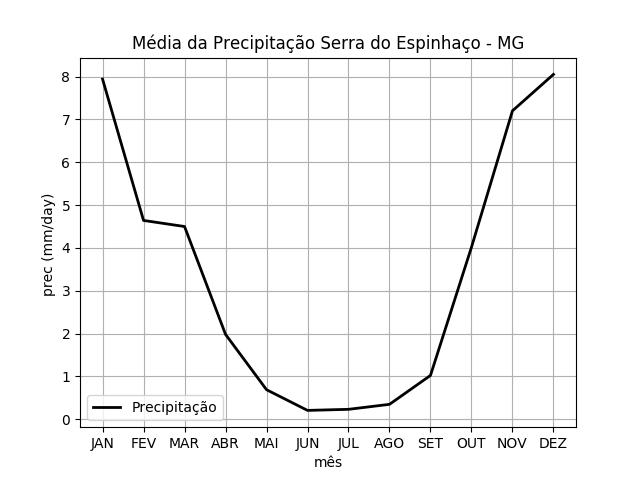
\includegraphics[width=0.4\paperwidth]{figuras/prec.png}}
\caption{Climatologia 10 anos da precipitação (mm/dia) para região da Serra do Espinhaço - MG}
\label{inputPrec}
\end{figure}

\begin{figure}[htbp]
\centerline{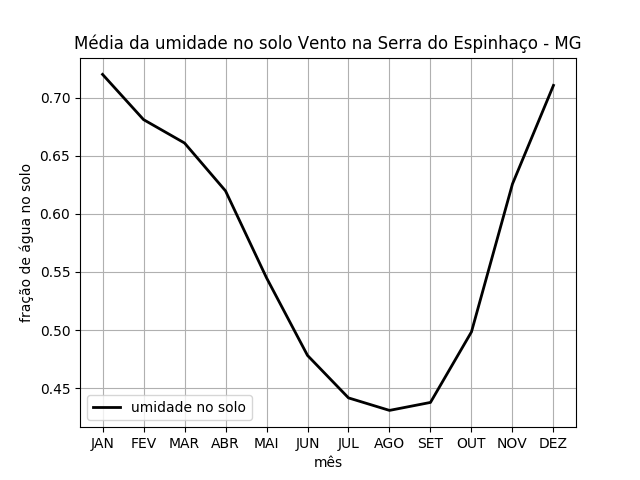
\includegraphics[width=0.4\paperwidth]{figuras/umidade.png}}
\caption{Climatologia 10 anos da umidade no solo (fração) para região da Serra do Espinhaço - MG}
\label{inputWsoi}
\end{figure}

\begin{figure}[htbp]
\centerline{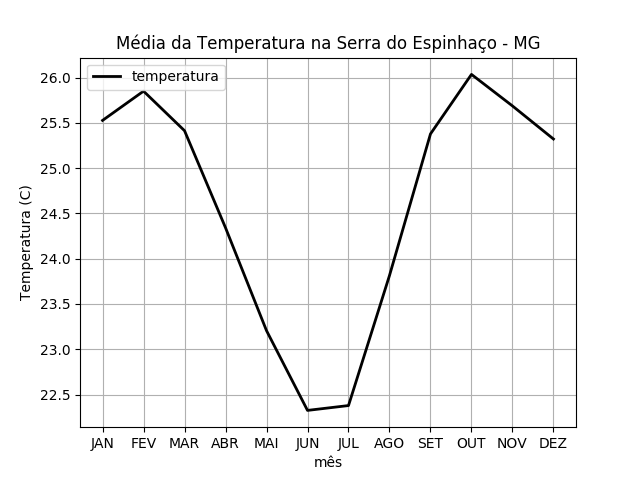
\includegraphics[width=0.4\paperwidth]{figuras/temp.png}}
\caption{Climatologia 10 anos da temperatura na superfície (C) para região da Serra do Espinhaço - MG}
\label{inputTemp}
\end{figure}


\begin{figure}[htbp]
\centerline{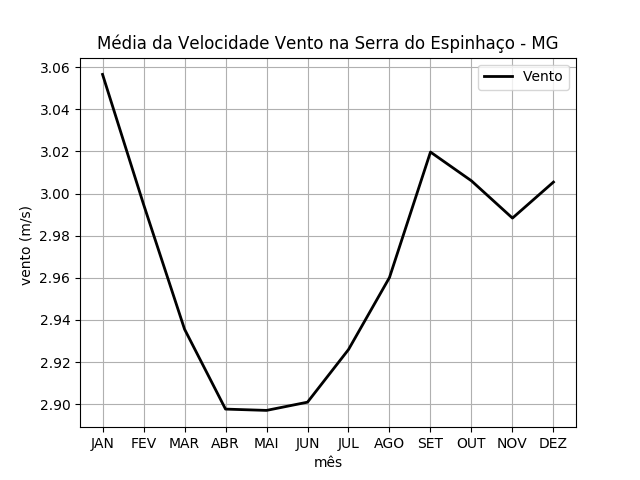
\includegraphics[width=0.4\paperwidth]{figuras/vento.png}}
\caption{Climatologia 10 anos da velocidade no vento (m/s) para região da Serra do Espinhaço - MG}
\label{inputVento}
\end{figure}

O mateiral combustivel florestal pode ser definido como qualquer material orgânico vivo ou morto, no solo e acima dele, capaz de entrar em ignição e queimar, entretanto a metéria verde(madeira e folhas de vegetação viva) possui uma difícil ignição pois possuem alto teor de umidade. Deste modo, para modelagem da RNA foi considarada apenas as informações de biomassa de serrapilheira, para a análise de dados de entrada da RNA, figura \ref{inputBioLit}.\\
\begin{figure}[htbp]
\centerline{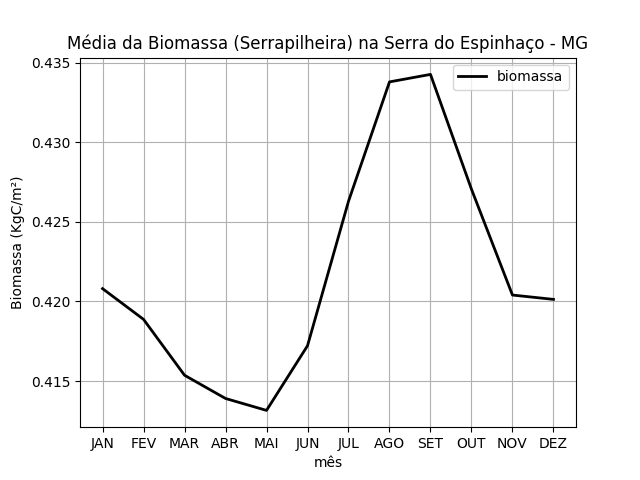
\includegraphics[width=0.4\paperwidth]{figuras/biomassa_litter.png}}
\caption{Climatologia 10 anos da Biomassa serrapilheira (Kg C/ m²) para região da Serra do Espinhaço - MG}
\label{inputBioLit}
\end{figure}
A Figura~\ref{inputNorm}, apresenta a comparação entre as vairáveis de entrada da RNA para as seguintes variáveis: preciptação e umidade no solo (que possuem correlação inversa com a o ocorrência de fogo), temperatura e velocidade de vento (onde o crescimento de ocorrencia de fogo coincidem com o aumento de valores de temperatura e velocidade de vento durante a seca), e quantidade de biomassa de serrapilheira.\\
\begin{figure}[htbp]
\centerline{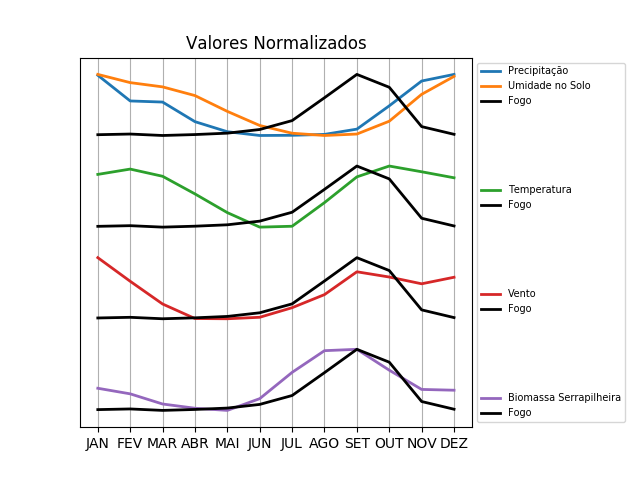
\includegraphics[width=0.44\paperwidth]{figuras/norm.png}}
\caption{Valores normalizados da climatologia 10 anos para: precipitação, umidade, vento e biomassa para região da Serra do Espinhaço - MG}
\label{inputNorm}
\end{figure}


%\begin{figure}[htbp]
%\centerline{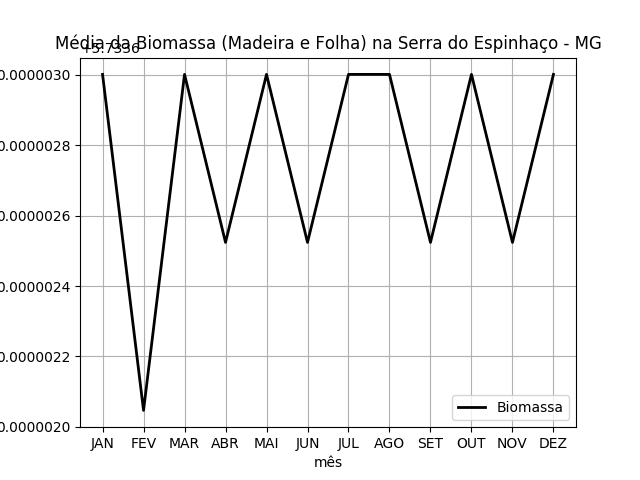
\includegraphics[width=0.4\paperwidth]{figuras/biomassa.png}}
%\caption{Variável de Entrada da RNA: climatologia 10 anos da Biomassa Madeira+Folha (Kg C/ m²) para região da Serra do Espinhaço - MG}
%\label{inputBioTot}
%\end{figure}
As Figuras~\ref{inputNorm} e \ref{inputNormFrac} apresenta a comparação das entradas normalizadas com as saídas esperadas.\\
A precipitação de chuva irá influênciar no umidade do solo, quanto mais seco for o ambiente maior será a periculosidade do material combustível florestal, as figuras~\ref{inputPrec} e \ref{inputWsoi} apresentam as medias dos valores e chuva e umidade no solo para a região da serra do espinhaço.\\
\begin{figure}[htbp]
\centerline{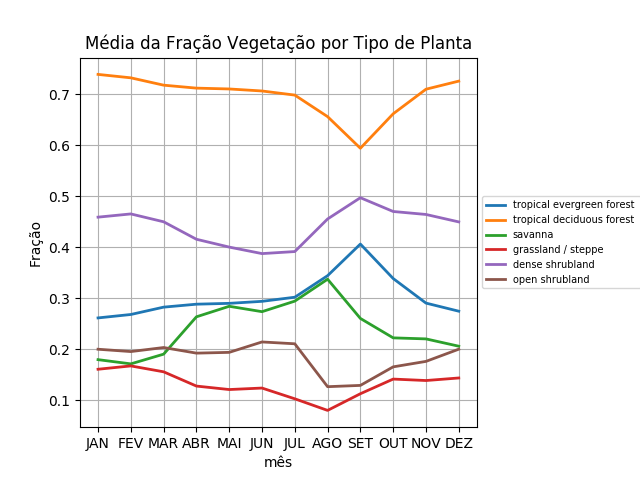
\includegraphics[width=0.44\paperwidth]{figuras/frac.png}}
\caption{Climatologia 10 anos da fração do tipo de vegetação existente na para região da Serra do Espinhaço - MG}
\label{inputFrac}
\end{figure}

Conforme Figura~\ref{inputNormFrac}, os picos de ocorrência de fogo coincidem com os maior índices de fração maior concentração de fração de vegetação do tipo floresta tropical e gramíneas esparsas,  e correlação inversa entre pastagem/estepes, e floresta topical decídua.\\
\begin{figure}[htbp]
\centerline{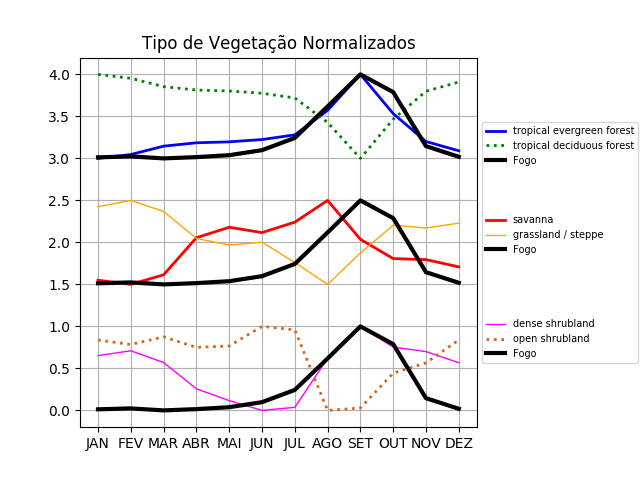
\includegraphics[width=0.44\paperwidth]{figuras/normveg.png}}
\caption{Valores normalizados da Climatologia 10 anos da fração do tipo de vegetação existente na para região da Serra do Espinhaço - MG}
\label{inputNormFrac}
\end{figure}


\section{Resultados e Discussão}
Conforme tabela 1  apresenta resultado boas aproximação dos valores calculados com 5 neurônios na camada oculta, os resultados obtdos com treinamento com acima de 5 neurônios na camada oculta, geram maior custo de tempo para treinamento sem aumento significavo nos resultados encontrados.\\


\begin{table}[htbp]
  \centering
  \begin{tabular}    {p{0.15\linewidth}p{0.15\linewidth}p{0.15\linewidth}}
    \hline
    Neuronio Camada Oculta & Erro médio quadrático & custo tempo\\
    \hline
    2 & 0.0078 & 23m18s\\
    3 & 0.0087 & 25m36s\\
    5 & 0.0069 & 27m54s\\
    10 & 0.0070 & 28m16s\\
    100 & 0.0067 & 32m31s\\
    \hline
  \end{tabular}
  \label{custoTempo}
  \caption{Custo de tempo para treinamento da RNA com diferentes números de neurônios e erro médio quadrático encontrado para 1000 épocas}
\end{table}


A Figura~\ref{resultados}  abaixo apresenta os resultados dos valores de ocorrência de fogo calculados pela RNA após o treinamento (simulado, em vermelho), e os valores de ocorrência de fogo observados a partir das detecções com o sensor MODIS (observado, em azul). Os valores correspondem às distribuições das médias mensais para toda a sub-região e período estudado. Conforme mostra a figura, as distribuições dos valores observados e simulados são em geral bem próximos. Os valores simulados são capazes de reproduzir a variação intra-anual típica para a região de estudo, onde os meses entre Agosto e Outubro apresentam os valores máximos, e os meses entre Novembro e Julho apresentam os valores mínimos. Outro aspecto interessante é que o range dos valores simulados também é próximo do range dos valores observados na maioria dos meses. No geral, porém, há também uma pequena tendência de sobre-estimativa de valores máximos na maior parte dos meses.
\begin{figure}[htbp]
\centerline{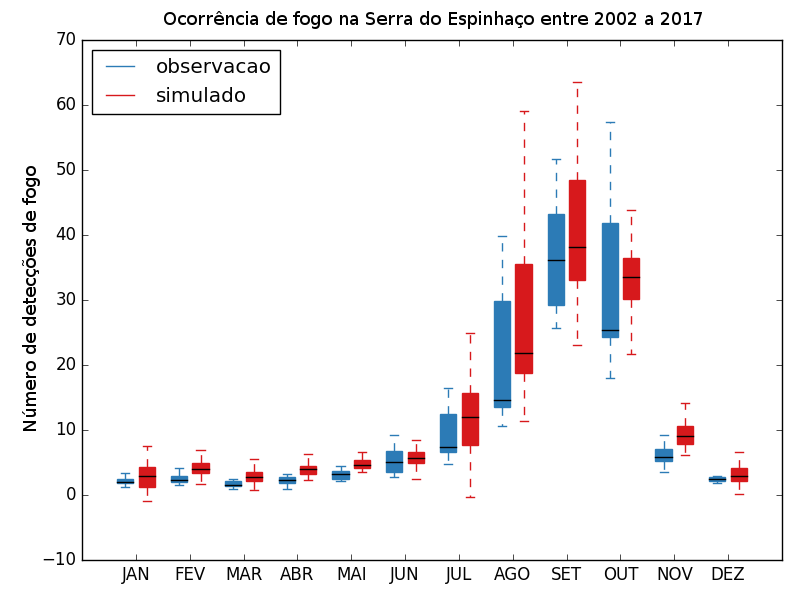
\includegraphics[width=0.42\paperwidth]{figuras/resultados.png}}
\caption{Comparação entre o número de detecções de fogo observado pelo sensor MODIS e simulado pela RNA entre 2002 e 2017 para a Serra do Espinhaço - MG.}
\label{resultados}
\end{figure}








\section{Conclusão}
Os resultados mostram que a RNA aqui desenvolvida  apresenta boa eficiência no cálculo de ocorrência do fogo na vegetação do Cerrado. As condições de ambientes geradas pelo INLAND para a sub-região da Serra do Espinhaço MG aliado a implementação da RNA em comparação aos dados do MODIS demonstram uma convergência satisfatória. Os valores simulados foram capazes de reproduzir o ciclo anual bem como o range dos valores medidos. Houve, porém, uma pequena tendência de sobre-estimativa de valores máximos na maior parte dos meses. Uma característica importante da metodologia e resultados é a possibilidade de aplicar RNAs para avaliar impactos de mudanças climáticas, e criar projetos ambientais que informem sobre possíveis alterações nos padrões do fogo. Para trabalhos futuros sugere-se também investir na utilização do presente método para uma área que contemple todo o Cerrado.



\begin{thebibliography}{00}

\bibitem{trends:ARRUDA}
ARRUDA, F. V.; SOUSA, D. G.; TERESA, F. B.; PRADO, V. H. M.; CUNHA, H. F.; IZZO, T. J.  \emph{Trends and gaps of the scientic literature about the effects of fire on Brazilian Cerrado.} Biota Neotropica.\hskip 1em plus
  0.5em minus 0.4em\relax 18(1): e20170426, 2018.

\bibitem{processes:FOLEY}
FOLEY, J. A.; PRENTICE, I. C.; RAMANKUTTY, N.; LEVIS, S.; POLLARD, D.; SITCH, S.; HAXELTINE, A. 
\emph{An integrated biosphere model of land surface processes, terrestrial carbon balance, and vegetation dynamics.} Global Biogeochemical Cycles, 1996.

\bibitem{rna:HAYKIN}
HAYKIN S.  \emph{Redes Neurais: princípios e práticas}, 2. ed. Porto Alegre, Bookman, 2001.


\bibitem{networks:KIMES}
KIMES, D. S.; NELSON, R. F.; MANRY, M. T.; FUNG, A. K.
\emph{ Attributes of neural networks for extracting continuous vegetation variables from optical and radar measurements.} International Journal of Remote Sensing, v.19, n.14, p.2639-2663, 1998.

\bibitem{biomass:MIRANDA}
MIRANDA, S. D.; BUSTAMANTE, M.; PALACE, M.; HAGEN, S.; KELLER, M.; FERREIRA, L. G. 
 \emph{Regional Variations in Biomass Distribution in Brazilian Savanna Woodland.} Biotropica, 46: 125-138. \hskip 1em plus
  0.5em minus 0.4em\relax doi:10.1111/btp.12095, 2014.

\bibitem{biodiversity:MYERS}
MYERS N.; MITTERMEIER R.A.; MITTERMEIER C.G.; DA FONSECA G.A.; Kent J.
\emph{Biodiversity hotspots for conservation priorities.} Nature, 403:853–858. doi: 10.1038/35002501, 2000.

\bibitem{landuse:NOBREGA}
NOBREGA, R. L. B.; GUZHA, A. C.; TORRES, G. N.; KOVACS, K.; LAMPARTER, G.; AMORIM, R. S. S. et al.
\emph{Effects of conversion of native cerrado vegetation to pasture on soil hydro-physical properties, evapotranspiration and streamflow on the Amazonian agricultural frontier.} PLoS ONE 12(6): e0179414, 2017.

\bibitem{RNA:Werbos}
WERBOS, P. J. \emph{Beyond regression: new tools for prediction and analysis in the behavioral sciences}, 1975. 

\end{thebibliography}

\end{document}
